\chapter{The Quantum Language of Astrophysical Radiation Mechanisms}
\label{chap:e16}

\begin{chapteropening}
By this point we have assembled a complete quantum toolkit for light: how many photons a mode contains on average (the Bose occupation number \(\bar n_\nu\) of Chapter~\ref{chap:e05}), what quantum state those photons form (the number, coherent, and thermal states of Chapter~\ref{chap:e06}), and how to tell the states apart using the second-order coherence function \(g^{(2)}\) (Chapter~\ref{chap:e08}). Now, for the first time, we truly point a telescope at the sky. A star, an HII region, a jet, a maser spot, a fast radio burst: each of them ultimately leaves an \(I_\nu\) spectrum on the detector; yet the photon-field statistics behind them can differ enormously. This chapter opens Part~4 of the book, and its task is a single sentence: to translate the whole zoo of astrophysical radiation mechanisms into the one language of ``mode occupation number + photon statistics,'' making clear which mechanisms are born as chaotic thermal light, which may deviate, and why capturing a genuinely nonclassical beam of light from an astrophysical source is so hard.
\end{chapteropening}

\section{Translating Radiation Mechanisms into Occupation Number and Photon Statistics}
\label{sec:e16-translation}

The traditional entry point to radiation mechanisms is the specific intensity \(I_\nu\), the radiant energy flux passing through per unit time, unit area, unit frequency, and unit solid angle, with CGS units \({\rm erg\,s^{-1}\,cm^{-2}\,Hz^{-1}\,sr^{-1}}\). If the source subtends a solid angle \(\Omega_{\rm s}\) on the sky, the flux density received by the telescope is approximately \(S_\nu\simeq I_\nu\,\Omega_{\rm s}\), commonly measured in Jy (\(1~{\rm Jy}=10^{-23}~{\rm erg\,s^{-1}\,cm^{-2}\,Hz^{-1}}\)). When textbooks treat radiation mechanisms, they usually stop at this spectrum \(I_\nu(\nu)\).

The trouble is that the spectrum is only an ``average.'' You can build the very same \(I_\nu\) spectrum out of completely different light fields. Picture two ponds whose surfaces ripple with waves of the same height: in one pond the ripples come from countless raindrops each splashing independently and adding incoherently; in the other, someone stands at the shore slapping the water rhythmically, so that many wave crests are pushed out in step. Standing far away and measuring the ``average ripple height,'' the two ponds look identical; but the moment you watch the way the surface \emph{fluctuates}, they part ways at once. Astrophysical radiation is the same: the mean spectrum \(I_\nu\) erases the correlations in photon arrival times, the correlations in polarization, and the joint probabilities among frequency channels, and it is precisely these that carry the fingerprint of the radiation mechanism.

To quantify these fingerprints, we recall the two coherence functions built up in the preceding two chapters. Let \(\hat E^{(+)}(t)\) be the positive-frequency electric-field operator (it corresponds to ``annihilating one photon,'' see Chapter~\ref{chap:e05}), and \(\hat E^{(-)}(t)=[\hat E^{(+)}(t)]^\dagger\). The normalized first-order coherence function is
\begin{equation}
  g^{(1)}(\tau)=
  \frac{\langle \hat E^{(-)}(t)\,\hat E^{(+)}(t+\tau)\rangle}
       {\langle \hat E^{(-)}(t)\,\hat E^{(+)}(t)\rangle},
  \label{eq:e16-g1}
\end{equation}
\begin{formulaexplain}
\(g^{(1)}(\tau)\) is the normalized first-order coherence function, dimensionless. The numerator correlates the field at the two instants \(t\) and \(t+\tau\); the denominator is the mean intensity. It measures how much the field's phase still ``remembers'' after a delay \(\tau\): \(|g^{(1)}|\) falls from 1 (fully coherent) to 0 (fully forgetful).
\end{formulaexplain}
The numerator \(\langle \hat E^{(-)}(t)\hat E^{(+)}(t+\tau)\rangle\) couples the field at the two instants, the denominator \(\langle \hat E^{(-)}(t)\hat E^{(+)}(t)\rangle\) is the mean intensity, and dividing one by the other gives a dimensionless quantity. \(|g^{(1)}(\tau)|\) decays from 1 at \(\tau=0\) to 0 at large \(\tau\), and the timescale of that decay is the coherence time \(\tau_c\simeq1/\Delta\nu\) (Chapter~\ref{chap:e02}). It governs the physics at the level of amplitude interferometry, line width, and visibility.

The second-order coherence function asks a different question, not ``does the phase still remember,'' but ``once one photon has arrived, will it bring another'':
\begin{equation}
  g^{(2)}(\tau)=
  \frac{\langle :\!\hat I(t)\,\hat I(t+\tau)\!:\rangle}{\langle \hat I(t)\rangle^2},
  \label{eq:e16-g2}
\end{equation}
\begin{formulaexplain}
\(g^{(2)}(\tau)\) is the normalized intensity correlation, dimensionless; \(\hat I(t)\) is the instantaneous intensity operator, and the colons denote normal ordering (annihilation operators placed to the right). It compares the joint probability of photon arrivals at the two instants against the independent case: \(>1\) bunching, \(=1\) Poisson, \(<1\) antibunching.
\end{formulaexplain}
Here \(\hat I(t)\propto\hat E^{(-)}(t)\hat E^{(+)}(t)\) is the instantaneous intensity, and the colons \(:\ :\) denote normal ordering (all \(\hat a^\dagger\) placed to the left of \(\hat a\), which removes the shot noise of the detection process itself, see Chapter~\ref{chap:e08}). \(g^{(2)}(\tau)\) is dimensionless, and its physics is a ``conditional probability'': given that a photon is detected at time \(t\), how much higher (relative to the independent case) is the probability of detecting another at \(t+\tau\): higher (\(>1\), bunching), the same (\(=1\), Poisson), or lower (\(<1\), antibunching, found only in nonclassical light).

Chapters~\ref{chap:e06} and~\ref{chap:e08} already worked out the value at \(\tau=0\) for three reference states, and we quote them here as known results: for a \emph{single-mode thermal (chaotic) state} \(g^{(2)}(0)=2\), for a \emph{coherent state} \(g^{(2)}(0)=1\), and for a \emph{number state} \(g^{(2)}(0)<1\). These are the three yardsticks of this chapter. The core work of the whole chapter is to place each astrophysical radiation mechanism between these three yardsticks: where does it fall by default? under what conditions does it deviate? and, most crucially, where will a real observation compress it to?

\section{Brightness Temperature: Converting Mean Intensity into Occupation Number}
\label{sec:e16-brightness}

Before we start translating mechanisms, we need a bridge that converts the directly observed \(I_\nu\) into the mode occupation number \(\bar n_\nu\) of Chapter~\ref{chap:e05}. That bridge is the \emph{brightness temperature} \(T_b\).

In the Rayleigh--Jeans form common in the radio and far-infrared, one inverts \(I_\nu\) into an ``equivalent temperature'':
\begin{equation}
  T_b=\frac{c^2\,I_\nu}{2k_B\nu^2}
      =\frac{c^2\,S_\nu}{2k_B\nu^2\,\Omega_{\rm s}} .
  \label{eq:e16-brightness-temperature}
\end{equation}
\begin{formulaexplain}
\(T_b\) is the brightness temperature, in K; \(c\) the speed of light, \(k_B\) the Boltzmann constant, \(\nu\) the frequency, \(\Omega_{\rm s}\) the source solid angle. It answers ``if this bit of radiation came from a blackbody in the R--J limit, how hot would that blackbody have to be.'' It is not the true temperature of the matter.
\end{formulaexplain}
Here \(c\) is the speed of light, \(k_B=1.38\times10^{-16}~{\rm erg\,K^{-1}}\) is the Boltzmann constant, and \(\nu\) is the frequency. The unit of \(T_b\) is K, but keep firmly in mind: it is a \emph{defined} equivalent quantity, answering the question ``if this \(I_\nu\) came from a Rayleigh--Jeans-limit blackbody, how hot would the blackbody be.'' For nonthermal electrons, masers, or FRBs, \(T_b\) is not at all equal to the thermal temperature of the matter; it can be higher than any physical temperature could ever reach. Note that \(T_b\propto S_\nu/\Omega_{\rm s}\): the smaller the source on the sky, the higher the \(T_b\) implied by the same flux density, so angular-size measurements (VLBI), variability timescales, and scattering broadening all feed directly into the mechanism judgment.

Now let us connect this bridge to the quantum side. The blackbody specific intensity for one polarization and one frequency mode is the Planck function \(B_\nu=(2h\nu^3/c^2)\,\bar n_\nu\), where the occupation number
\[
  \bar n_\nu=\frac{1}{\exp(h\nu/k_BT)-1}
\]
is precisely the protagonist of Chapter~\ref{chap:e05}. Substituting \(I_\nu=B_\nu\) into the brightness-temperature definition~\eqref{eq:e16-brightness-temperature}, the \(2\nu^2/c^2\) on both sides cancels, and we obtain directly an extremely clean correspondence:
\begin{equation}
  \bar n_\nu=\frac{k_B T_b}{h\nu}
  \qquad(\text{exact under the Rayleigh--Jeans definition}).
  \label{eq:e16-occupation-from-tb}
\end{equation}
\begin{formulaexplain}
\(\bar n_\nu\) is the mean photon number in a single spacetime--polarization mode; \(k_B T_b\) is the energy corresponding to the brightness temperature, and \(h\nu\) is the single-photon energy. This equation says: \emph{brightness temperature is essentially the occupation number}, the two differing only by the conversion factor \(h\nu/k_B\).
\end{formulaexplain}
This step is the ``Rosetta Stone'' of the chapter: \(\bar n_\nu=k_B T_b/(h\nu)\). Brightness temperature is nothing but the mode occupation number wearing a ``temperature'' coat. High \(T_b\) means every mode is stuffed with photons; low \(T_b\) means the modes are nearly empty. In one glance this welds the ``mean spectrum'' to the ``quantum occupation number.''

Plug in two real numbers and the sense of scale comes out at once. First, the \emph{stellar photosphere in the visible}: taking \(T\simeq6000~{\rm K}\) and \(\nu\simeq6\times10^{14}~{\rm Hz}\) (\(\lambda\simeq500~{\rm nm}\)), we get \(h\nu/k_BT=(6.6\times10^{-27}\times6\times10^{14})/(1.38\times10^{-16}\times6000)\simeq4.8\), which lies in the Wien regime rather than the R--J regime, giving occupation number \(\bar n_\nu=1/(e^{4.8}-1)\simeq0.008\). On average, each mode holds only a hundredth of a photon! This explains why the visible light of a star is an extremely ``dilute'' beam, why the Hanbury Brown--Twiss bunching signal is so faint, and why the photon rate is the lifeline of interstellar measurements (Chapter~\ref{chap:e10}). Second, the \emph{FRB}: a millisecond, Jy-level, Gpc-distance, GHz-frequency radio pulse, substituted into~\eqref{eq:e16-brightness-temperature}, gives
\begin{equation}
  T_b\simeq
  1.1\times10^{35}~{\rm K}
  \left(\frac{S_\nu}{1~{\rm Jy}}\right)
  \left(\frac{D_A}{1~{\rm Gpc}}\right)^2
  \left(\frac{t_{\rm FRB}}{1~{\rm ms}}\right)^{-2}
  \left(\frac{\nu}{1~{\rm GHz}}\right)^{-2},
  \label{eq:e16-frb-tb}
\end{equation}
\begin{formulaexplain}
\(S_\nu\) the pulse flux density, \(D_A\) the angular-diameter distance, \(t_{\rm FRB}\) the pulse width, \(\nu\) the observing frequency. This astronomical number shows that the brightness temperature of a millisecond FRB far exceeds the upper limit any incoherent radiation can reach.
\end{formulaexplain}
where \(D_A\) is the angular-diameter distance (the pulse width \(t_{\rm FRB}\) sets an upper bound on the source size through the causality limit \(\Omega_{\rm s}\lesssim(c\,t_{\rm FRB}/D_A)^2\)). Substituting \(T_b\sim10^{35}~{\rm K}\) and \(\nu=1~{\rm GHz}\) into~\eqref{eq:e16-occupation-from-tb}: \(\bar n_\nu\simeq k_BT_b/(h\nu)=(1.38\times10^{-16}\times10^{35})/(6.6\times10^{-27}\times10^{9})\simeq2\times10^{36}\). Each mode is crammed with \(10^{36}\) photons; this can no longer be explained by ``many independent particles each radiating on their own''; it requires an enormous number of charged particles to \emph{cooperatively} emit on scales smaller than a wavelength or with controlled phase \citep{2007Sci...318..777L,2019A&ARv..27....4P,2022A&ARv..30....2P}. Here the occupation number shouts the word ``coherence'' on our behalf.

\begin{figure}[tbp]
\centering
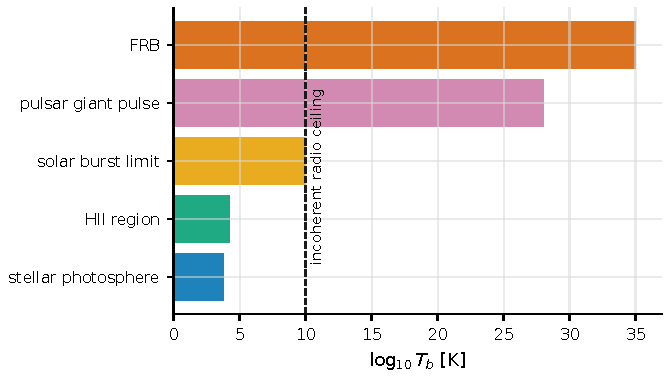
\includegraphics[width=0.82\linewidth]{figures/generated/chapter_09/ch09_brightness_temperature_scale.pdf}
\caption{Brightness temperature as the first-level criterion for radiation mechanisms. Stellar photospheres and HII regions fall in the ordinary thermal-temperature range (corresponding to occupation number \(\bar n_\nu\lesssim1\)); solar and stellar radio bursts exceeding \(10^{10}~{\rm K}\) often require a coherent mechanism; the brightness temperatures of pulsar giant pulses and FRBs are higher still (occupation number up to \(10^{30}\) and beyond) and can only be explained by coherent emission or strong beaming geometry. The dashed line marks the order of magnitude of the commonly used incoherent-radio limit.}
\label{fig:e16-brightness-temperature}
\end{figure}

Brightness temperature gives us a hard, empirical threshold. Dulk's review of solar and stellar radio emission provides a practical criterion: the \(T_b\) of incoherent radio emission can hardly exceed \(10^9\)--\(10^{10}~{\rm K}\), an upper limit set mainly by gyrosynchrotron self-absorption and energetic constraints (once the occupation number is too high, self-absorption and radiation reaction push it back down; incidentally, the inverse-Compton catastrophe of Kellermann--Pauliny-Toth gives a higher scale of \(\sim10^{12}~{\rm K}\), and the two should not be confused); bursts significantly above this range must invoke a coherent mechanism, such as plasma emission or the electron-cyclotron maser \citep{1985ARA&A..23..169D}. The brightness-temperature yardstick (Figure~\ref{fig:e16-brightness-temperature}) thus becomes the first cut in mechanism judgment: is the occupation number the \(\lesssim1\) of ``dilute thermal light,'' or the \(10^{20}\), \(10^{30}\) of a ``coherent burst''? But this is only the first cut: it only checks whether the mean energy density is reasonable, and says nothing about whether these photons add up independently or emit cooperatively. To settle that step, we must call upon photon statistics.

\section{Why Thermal Radiation Is Born as Chaotic Light}
\label{sec:e16-thermal}

Consider first the most ``well-behaved'' entry in the family tree: thermal radiation. Stellar photospheres, dust, HII regions, and the cosmic microwave background are all approximately in local thermodynamic equilibrium. Their mode occupation numbers are given by the Planck distribution,
\begin{equation}
  \bar n_\nu=\frac{1}{\exp(h\nu/k_BT)-1},
  \label{eq:e16-planck-occupation}
\end{equation}
\begin{formulaexplain}
\(\bar n_\nu\) the mean occupation number of the mode at frequency \(\nu\); \(h\nu\) the single-photon energy, \(T\) the temperature of the matter. In the R--J regime (\(h\nu\ll k_BT\)), \(\bar n_\nu\approx k_BT/h\nu\gg1\); in the Wien regime (\(h\nu\gg k_BT\)), \(\bar n_\nu\approx e^{-h\nu/k_BT}\ll1\).
\end{formulaexplain}
Here \(T\) is the thermal temperature of the matter. Note that the visible light of a stellar photosphere often lies in the Wien regime (\(h\nu/k_BT>1\)), so color temperature, effective temperature, and brightness temperature must not be conflated: for the same star, \(\bar n_\nu\) is large at the radio end and small at the optical end. But whichever regime it falls in, the \emph{statistical properties} of the thermal state are the same, and this is precisely what we care about.

Why is thermal radiation born as chaotic light? The physical picture is this: a thermal source contains an enormous number of independent emitters (atoms, ions, electrons), each emitting a small wave train at a random time with a random phase. The total electric field reaching the detector is the vector sum of these millions upon millions of little arrows with random phases and random amplitudes. Here the central limit theorem enters (the sum of a large number of independent random quantities tends to a Gaussian distribution), so within a narrow band the complex electric field \(\hat E^{(+)}(t)\) is a \emph{complex Gaussian random process}. This is no coincidence; it is the inevitable consequence of ``adding up many independent events.''

A Gaussian random process has a beautiful algebraic property (proved in Chapter~\ref{chap:e08}, quoted here as a known result): its fourth-order moment can be decomposed into products of second-order moments (the moment theorem / Gaussian moment theorem). Applying this property to the numerator of~\eqref{eq:e16-g2} yields the Siegert relation
\begin{equation}
  g^{(2)}(\tau)=1+\frac{|g^{(1)}(\tau)|^2}{M_{\rm eff}},
  \label{eq:e16-siegert}
\end{equation}
\begin{formulaexplain}
The Siegert relation: the second-order coherence of chaotic (Gaussian) light is fully determined by its first-order coherence. \(M_{\rm eff}\) is the number of modes averaged over simultaneously. The single-mode case (\(M_{\rm eff}=1\), \(\tau=0\)) gives \(g^{(2)}(0)=1+1=2\), the thermal-light bunching peak.
\end{formulaexplain}
In a single spacetime--polarization mode (\(M_{\rm eff}=1\)) at \(\tau=0\), since \(|g^{(1)}(0)|=1\), we immediately obtain \(g^{(2)}(0)=1+1=2\). This is the seed of thermal-light bunching, and the anchor point we will use again and again in this chapter: \emph{as long as it is ``many independent emitters added together,'' the light field is a Gaussian chaotic field, and it automatically carries the \(g^{(2)}(0)=2\) bunching peak.} Thermal light is not mysterious; its bunching is purely the statistical consequence that ``the intensity clumps and fluctuates'' when random-phase amplitudes superpose.

The power of this logic lies in its \emph{indifference to mechanism}. As long as ``many independent events add up and the phase is random within a narrow band'' is satisfied, the shape of the spectrum is irrelevant: the conclusion is always Gaussian chaotic light. The first example is \emph{free-free radiation} (bremsstrahlung): it is not the blackbody spectrum itself but the continuous spectrum from countless electrons being accelerated in the Coulomb fields of ions, each emitting one burst of braking radiation. The phase of a single collision is completely unpredictable, and the complex field within a narrow band still tends to a Gaussian process. In a thin ionized gas, the emission coefficient scales as
\begin{equation}
  j_\nu^{\rm ff}\propto
  n_e\,n_i\,T_e^{-1/2}
  \exp\!\left(-\frac{h\nu}{k_BT_e}\right)
  g_{\rm ff}(\nu,T_e),
  \label{eq:e16-free-free}
\end{equation}
\begin{formulaexplain}
\(j_\nu^{\rm ff}\) the free-free emission coefficient; \(n_e,n_i\) the electron and ion number densities (\({\rm cm^{-3}}\)), \(T_e\) the electron temperature, \(g_{\rm ff}\) the Gaunt factor (\(\sim1\) to a few tens). It is a continuous spectrum contributed by many independent Coulomb collisions.
\end{formulaexplain}
where \(n_e,n_i\) are the electron and ion number densities (\({\rm cm^{-3}}\)), \(T_e\) is the electron temperature, and \(g_{\rm ff}\) is the Gaunt factor. HII regions have \(T_e\sim10^4~{\rm K}\); stellar winds and accretion flows can be hotter. The spectral shape (nearly flat at the radio end, exponentially declining at high frequency) is completely different from a blackbody, but the photon statistics are the same chaotic thermal light, likewise carrying the seed \(g^{(2)}(0)=2\).

Still, for the spectrum to be observed it must pass through the medium, which brings in the radiative transfer equation:
\begin{equation}
  \frac{{\rm d}I_\nu}{{\rm d}s}=j_\nu-\alpha_\nu I_\nu,
  \qquad
  S_\nu=\frac{j_\nu}{\alpha_\nu}.
  \label{eq:e16-radiative-transfer}
\end{equation}
\begin{formulaexplain}
\({\rm d}I_\nu/{\rm d}s\) the change of intensity along the line of sight; \(j_\nu\) adds radiation, \(\alpha_\nu I_\nu\) absorbs it, and \(S_\nu=j_\nu/\alpha_\nu\) is the source function. It links the emission mechanism to the optical depth.
\end{formulaexplain}
\(s\) is distance along the line of sight, \(j_\nu\) is the emission coefficient, \(\alpha_\nu\) is the absorption coefficient, and the source function is \(S_\nu=j_\nu/\alpha_\nu\). Defining the optical depth \({\rm d}\tau_\nu=\alpha_\nu\,{\rm d}s\) and integrating~\eqref{eq:e16-radiative-transfer} over a uniform slab (this is a first-order linear ODE, solved directly with the integrating factor \(e^{\tau_\nu}\), a standard result), then converting to brightness temperature, we get
\begin{equation}
  T_b=T_{\rm eff}\left(1-e^{-\tau_\nu}\right)+T_{\rm bg}\,e^{-\tau_\nu}.
  \label{eq:e16-tb-transfer}
\end{equation}
\begin{formulaexplain}
\(T_b\) the emergent brightness temperature; \(T_{\rm eff}\) the temperature corresponding to the source function, \(T_{\rm bg}\) the background brightness temperature, \(\tau_\nu\) the optical depth. A thin source (\(\tau_\nu\ll1\)) adds only a little; a thick source (\(\tau_\nu\gg1\)) tends toward its own source function.
\end{formulaexplain}
For small optical depth \(T_b\simeq T_{\rm eff}\tau_\nu+T_{\rm bg}\) (a thin source contributes only a small increment), and for large optical depth \(T_b\to T_{\rm eff}\) (a thick source thermalizes to its own source function). This equation is commonly used to judge whether a source is thermalized, semi-transparent, or nonthermal-dominated \citep{1979rpa..book.....R,2011piim.book.....D,1985ARA&A..23..169D}. It also explains where the brightness-temperature upper limit comes from: once the optical depth is large enough, \(T_b\) is pinned by the source function (for a thermal source, the matter temperature) and cannot climb higher.

To summarize the physics of this section: what thermal and free-free radiation have in common is not the spectral shape but the statistical root of ``many independent emitters added together.'' This root makes their fields Gaussian chaotic fields, both sitting by default at \(g^{(2)}(0)=2\). This is our ``zero point'': every other mechanism that follows will be measured by whether it stays at this setting or deviates from it.

\section{Nonthermal Particles: Spectrum and Polarization Change, but the Statistics Often Do Not}
\label{sec:e16-nonthermal}

One of the easiest mistakes a beginner makes is to equate ``nonthermal'' with ``non-Gaussian statistics.'' This section is devoted to dispelling that. Synchrotron and inverse-Compton radiation: their \emph{spectrum and polarization} do indeed depart completely from a blackbody, but their \emph{photon statistics} are for the most part still Gaussian chaotic light. The reason is again that same root: as long as the emitters are many independent particles with random phase within a narrow band, the central limit theorem still compresses the field into a Gaussian process.

Synchrotron radiation comes from relativistic electrons spiraling in a magnetic field. The characteristic frequency of a single electron is
\begin{equation}
  \nu_c=\frac{3eB\sin\alpha}{4\pi m_ec}\,\gamma^2 ,
  \label{eq:e16-synch-critical}
\end{equation}
\begin{formulaexplain}
\(\nu_c\) the synchrotron characteristic frequency; \(e\) the elementary charge, \(B\) the magnetic field, \(\alpha\) the pitch angle, \(m_e\) the electron mass, \(\gamma\) the Lorentz factor. The frequency grows with \(B\) and \(\gamma^2\), so high-energy electrons can push the radiation to very high frequency bands.
\end{formulaexplain}
where \(e\) is the elementary charge, \(B\) the magnetic field strength, \(\alpha\) the pitch angle, \(m_e\) the electron mass, and \(\gamma\) the Lorentz factor. A word of caution: the bare symbol \(\alpha\) here refers specifically to the pitch angle (the angle between the electron velocity and the magnetic field); do not confuse it with the absorption coefficient \(\alpha_\nu\) of the previous section or the synchrotron spectral index \(\alpha_{\rm syn}\) that appears below; the three are distinguished by context and subscript. Plug in numbers: \(B=1~{\rm G}\), \(\gamma=10^3\), \(\sin\alpha=1\) gives \(\nu_c\simeq4.2\times10^{12}~{\rm Hz}\) (far-infrared); switching to the weak fields of intergalactic or jet scales, \(B=10^{-5}~{\rm G}\), the same electrons radiate mainly in the radio. The emission coefficient of a real source is the superposition of contributions from electrons of all energies,
\begin{equation}
  j_\nu^{\rm syn}=\int P_\nu(E,B,\alpha)\,N(E)\,{\rm d}E ,
  \label{eq:e16-synch-emissivity}
\end{equation}
\begin{formulaexplain}
\(j_\nu^{\rm syn}\) the synchrotron emission coefficient; \(P_\nu\) the single-electron power spectrum, \(N(E)\) the electron energy distribution. The integral shows that the observed spectrum is the sum of contributions from electrons of all energies: precisely ``many independent emitters added together.''
\end{formulaexplain}
If the electron energy spectrum is a power law \(N(E)\propto E^{-p}\), optically thin synchrotron radiation gives a power-law spectrum \(I_\nu\propto\nu^{-\alpha_{\rm syn}}\) with spectral index \(\alpha_{\rm syn}=(p-1)/2\). The signature of synchrotron radiation is high linear polarization: in a uniform field the maximum linear polarization degree is
\begin{equation}
  \Pi_{\rm syn}=\frac{p+1}{p+7/3}.
  \label{eq:e16-synch-polarization}
\end{equation}
\begin{formulaexplain}
\(\Pi_{\rm syn}\) the maximum linear polarization degree of optically thin synchrotron radiation; \(p\) the electron energy-spectrum index. It is the theoretical upper limit of polarization under a uniform field with a power-law electron distribution.
\end{formulaexplain}
For example, at \(p=2.4\) we have \(\Pi_{\rm syn}\simeq72\%\). In real jets, supernova remnants, and pulsar wind nebulae the polarization is often much lower, because a disordered field direction, Faraday rotation, beam averaging, and the superposition of multiple emission regions all cancel polarization. Note the key point: the integral sign in~\eqref{eq:e16-synch-emissivity} itself says ``many independent electrons added together,'' so \emph{even though the spectrum is a power law and the polarization is high, the field is still approximately a Gaussian chaotic field, and \(g^{(2)}(0)\) still defaults to 2}. Synchrotron radiation rewrites the mean spectrum and polarization (determined by the nonthermal electron distribution and the field geometry); it does not rewrite the photon-statistics setting \citep{1965ARA&A...3..297G,1970RvMP...42..237B,1978bllo.conf..328B,2012ApJ...752..157Z}.

Inverse-Compton scattering kicks low-energy seed photons up to high energy. In the Thomson limit, the scattered photon energy scales as
\begin{equation}
  h\nu_{\rm IC}\sim\gamma^2\,h\nu_{\rm seed}.
  \label{eq:e16-ic-energy}
\end{equation}
\begin{formulaexplain}
\(h\nu_{\rm seed}\) the seed-photon energy, \(h\nu_{\rm IC}\) the scattered energy, \(\gamma\) the electron Lorentz factor. In the Thomson limit a single scattering boosts the photon energy by roughly \(\gamma^2\).
\end{formulaexplain}
Multiple scatterings in a hot electron cloud are measured by the Compton \(y\) parameter:
\begin{equation}
  y\simeq4\,\frac{k_BT_e}{m_ec^2}\,\max(\tau_T,\tau_T^2),
  \label{eq:e16-compton-y}
\end{equation}
\begin{formulaexplain}
\(y\) the Comptonization strength parameter; the prefactor \(4k_BT_e/m_ec^2\) is the fractional energy gain per scattering, and \(\max(\tau_T,\tau_T^2)\) estimates the mean number of scatterings (\(\tau_T\) the Thomson optical depth). It judges how much the spectrum is rewritten by the electron cloud.
\end{formulaexplain}
For \(y\ll1\) the spectrum is only slightly modified; for \(y\sim1\) a clear Comptonized continuum forms; for \(y\gg1\) it tends toward saturated Comptonization. In X-ray binaries, AGN coronae, and GRB photospheric models, the mean spectrum is often a blend of synchrotron, thermal photon, and inverse-Compton components, and the spectral index alone can hardly pin down the mechanism uniquely \citep{1980A&A....86..121S,1999MNRAS.309..496G,2013ApJ...765..103L}. And these scattering processes still involve an enormous number of independent photon--electron events, so the statistics of the output light field remain at the chaotic-thermal-light setting.

\begin{figure}[tbp]
\centering
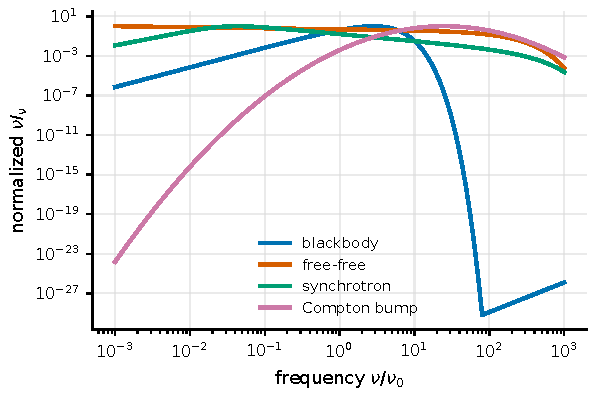
\includegraphics[width=0.84\linewidth]{figures/generated/chapter_09/ch09_spectral_mechanisms.pdf}
\caption{Schematic of the normalized spectral shapes of common continuum radiation mechanisms. A blackbody has a thermal peak and an R--J low-frequency end; free-free radiation is nearly flat in the radio and declines exponentially at high frequency; synchrotron radiation, from a nonthermal electron energy spectrum, gives a power law with low- and high-frequency cutoffs; the inverse-Compton component often appears as a high-energy bump. The four spectral shapes are wildly different, but as long as it is ``many independent particles added together,'' the photon statistics default to the chaotic-thermal-light setting \(g^{(2)}(0)=2\).}
\label{fig:e16-spectral-mechanisms}
\end{figure}

The pedagogical takeaway of this section, in one sentence: \emph{spectrum and polarization can tell you the particle distribution and the field geometry, but they cannot tell you the photon statistics.} Thermal, free-free, synchrotron, inverse-Compton: the spectral shape changes all the way from a thermal peak to a power law to a high-energy bump (Figure~\ref{fig:e16-spectral-mechanisms}), yet they share the same statistical root and are all Gaussian chaotic light. To make \(g^{(2)}\) genuinely deviate from 2, one must break the premise of ``many independent emitters added together,'' and this drives us to the coherent mechanisms of the next section.

\section{Coherent Mechanisms: The Few Exits That Break the Brightness-Temperature Ceiling}
\label{sec:e16-coherent}

To deviate from chaotic thermal light there is only one road: make the emitters no longer independent, let a large number of charges \emph{cooperate} in phase. Once they cooperate, the premise of the central limit theorem collapses, the field is no longer a Gaussian process, the occupation number can shoot up to \(10^{20}\), \(10^{30}\), and the brightness temperature breaks through the incoherent ceiling of \(10^{10}~{\rm K}\). The mechanisms that achieve this in astrophysical sources can be counted on one's fingers, and this section names them one by one.

\paragraph{Stimulated-emission class: masers and lasers.}
\label{sec:e16-maser}

The maser starts from ``negative absorption.'' If a population inversion appears on some spectral line (the upper level more populated than the lower), the absorption coefficient becomes negative, \(\alpha_\nu<0\). Substituted into radiative transfer, the intensity is \emph{exponentially amplified} along the path:
\begin{equation}
  I_\nu(L)\simeq I_\nu(0)\,\exp(|\tau_m|),
  \qquad
  \tau_m=\int_0^L\alpha_\nu\,{\rm d}s<0 .
  \label{eq:e16-maser-gain}
\end{equation}
\begin{formulaexplain}
\(I_\nu(0),I_\nu(L)\) the intensity before and after the path; \(\tau_m<0\) the negative-absorption optical depth. When unsaturated, the gain grows exponentially with \(|\tau_m|\): this is the source of high-brightness-temperature narrow lines.
\end{formulaexplain}
When unsaturated, the gain is exponentially sensitive to the optical depth and can push \(T_b\) extremely high; after saturation, stimulated emission depletes the inversion, and line width, polarization, and intensity are all taken over by the pump and geometry. Water masers, OH masers, and SiO masers can reach extremely high brightness temperatures, and the occupation number is therefore huge. But take care: the coherence of astrophysical masers is usually determined jointly by many velocity-coherent paths, turbulent clumps, and polarization propagation effects, and \emph{cannot} be simply equated with the near-coherent state of a single-mode laser beam in the laboratory. The work of Goldreich, Keeley, Kwan, and Elitzur gives the basic constraints on source size, saturation, line width, and polarization \citep{1972ApJ...174..517G,1973ApJ...179..111G,1974ApJ...190...27G,1982RvMP...54.1225E,1992ARA&A..30...75E}. Stimulated emission is not limited to the radio either: in the Weigelt blobs of Eta Carinae, Fe II and O I lines can, under particular pumping and optical depth, show laser or laser-like amplification, whose line width, position, polarization, and photon correlations can test the inversion and feedback geometry \citep{2004A&A...428..497J,2005NewA...10..361J,2008AIPC..984..216D}. As long as the pumping, level structure, and escape path are suitable, optical spectral lines too can carry statistical signatures distinct from ordinary thermal light.

The electron-cyclotron maser is a coherent radio mechanism in strongly magnetized, low-density plasma. It requires the electron distribution to depart from equilibrium (e.g., a loss-cone distribution), and requires the relation between the cyclotron frequency and the plasma frequency to allow the electromagnetic wave to escape. The cyclotron frequency is
\begin{equation}
  \nu_B=\frac{eB}{2\pi m_ec}
       \simeq2.8~{\rm MHz}\left(\frac{B}{1~{\rm G}}\right).
  \label{eq:e16-cyclotron-frequency}
\end{equation}
\begin{formulaexplain}
\(\nu_B\) the electron-cyclotron frequency; \(e\) the charge, \(B\) the magnetic field, \(m_e\) the electron mass. The observed maser frequency can be used to infer the order of magnitude of the field in the emission region.
\end{formulaexplain}
If one sees the fundamental or a low harmonic of the electron-cyclotron maser at GHz frequency, the field is of order a few hundred G to a few kG. High-circular-polarization radio bursts from the Sun, planets, brown dwarfs, and low-mass stars can all fall into this framework \citep{1982ApJ...259..844M,2006A&ARv..13..229T,2008ApJ...684..644H,1985ARA&A..23..169D}.

\paragraph{Antenna class: coherent curvature radiation.}
\label{sec:e16-curvature}

Curvature radiation demonstrates another road to coherence: it relies not on level inversion but on making many charges move cooperatively in phase, like an antenna. When a relativistic charge moves along a curved magnetic field line, the characteristic frequency and power of a single charge are
\begin{equation}
  \nu_{\rm curv}=\frac{3c}{4\pi\rho}\gamma^3,
  \qquad
  P_{\rm curv}=\frac{2e^2c}{3\rho^2}\gamma^4 ,
  \label{eq:e16-curvature}
\end{equation}
\begin{formulaexplain}
\(\nu_{\rm curv}\) the curvature-radiation characteristic frequency, \(P_{\rm curv}\) the single-particle power; \(\rho\) the radius of curvature of the field line, \(\gamma\) the Lorentz factor. Coherent curvature radiation additionally requires many charges to be phase-synchronized.
\end{formulaexplain}
where \(\rho\) is the radius of curvature of the field line. Plug in numbers: \(\rho=10^7~{\rm cm}\), \(\gamma=300\); compute first the prefactor \(3c/(4\pi\rho)\simeq7.2\times10^2~{\rm Hz}\), then multiply by \(\gamma^3=2.7\times10^7\) to get \(\nu_{\rm curv}\sim2\times10^{10}~{\rm Hz}\) (still in the radio/microwave band). The curvature radiation of a single particle is too weak; coherent curvature radiation requires many charges to bunch on a longitudinal scale smaller than a wavelength, so that the field amplitudes \emph{add} rather than the powers, and the total power grows roughly as the \emph{square} of the particle number. This is the essence of the ``antenna'': if \(N\) charges are phase-synchronized, the radiated power \(\propto N^2\) rather than \(N\). This idea has long been used for pulsar coherent radio emission and has also been carried into FRB models \citep{1977ApJ...212..800C,2018MNRAS.477.2470L}.

FRBs push the coherent mechanism to the extreme. The Lorimer burst provided the first set of evidence for millisecond timescale, cold-plasma dispersion, and \(T_b\sim10^{34}~{\rm K}\); repeaters and the CHIME sample show that repetition, polarization, frequency drift, microstructure, and host environment all enter the models; and the 2020 event from SGR 1935+2154 directly connected a Galactic magnetar to FRB-like radio bursts \citep{2007Sci...318..777L,2019A&ARv..27....4P,2022A&ARv..30....2P,2020Natur.587...54C,2020Natur.587...59B}. The many models fall roughly into two classes: maser-type, relying on population inversion or shocks, and antenna/curvature-type, relying on charge bunches or current sheets. Sub-microsecond structure, strong polarization, frequency drift, and multiband non-detections jointly constrain the emission radius, Lorentz factor, plasma density, and radiation efficiency.

The physical landing point of this section: coherent mechanisms can break the brightness-temperature ceiling and push the occupation number to astronomical numbers because they break the premise of ``independent emitters added together'' and make the charges cooperate. Their photon statistics can \emph{in principle} deviate from chaotic thermal light, but remember, the deviation spoken of here refers to the signature of stimulated/cooperative emission at extremely high occupation numbers, and is not the same as the squeezed, antibunched nonclassical light we pursue in the laboratory. Genuine nonclassical light requires \(g^{(2)}(0)<1\), and in astrophysical sources, even if the source itself has deviated from thermal statistics, whether we can \emph{measure} that deviation must still pass the test of the next section.

\section{Why It Is Extremely Hard to Isolate Genuinely Nonclassical Light in Astrophysical Sources}
\label{sec:e16-dilution}

Now we reach the most crucial, and also the most easily romanticized, point of the chapter. We have said that single-mode thermal light has \(g^{(2)}(0)=2\) and that coherent mechanisms may deviate, which sounds as though one need only set up a detector to read out the mechanism's fingerprint. Real observations, however, almost always \emph{smooth over} these fingerprints. What smooths them is ``mode dilution.''

The physical picture: that beautiful bunching peak of \(g^{(2)}(0)=2\) holds only in a \emph{single} spacetime--polarization mode. But a real telescope collects a great many modes at once: the telescope's receiving aperture covers many spatial coherence patches (spatial modes \(M_{\rm sp}\)), it is sensitive to both polarizations (polarization modes \(M_{\rm pol}\)), and its time resolution \(\Delta t\) is far broader than the coherence time \(\tau_c\) (temporal modes \(\sim\Delta t/\tau_c\)). The fluctuations of these modes are mutually independent, and once averaged, the bunching peak is diluted. Writing out \(M_{\rm eff}\) in the Siegert relation~\eqref{eq:e16-siegert} in detail,
\begin{equation}
  g^{(2)}_{\rm meas}(0)-1\simeq\frac{1}{M_{\rm eff}},
  \qquad
  M_{\rm eff}\simeq M_{\rm sp}\,M_{\rm pol}\left(1+\frac{\Delta t}{\tau_c}\right).
  \label{eq:e16-mode-dilution}
\end{equation}
\begin{formulaexplain}
\(M_{\rm eff}\) the effective number of mixed modes; \(M_{\rm sp},M_{\rm pol}\) the numbers of spatial and polarization modes, \(\Delta t/\tau_c\) the averaging of the time bin over the coherence time. The more modes there are, the lower the measurable bunching contrast \(g^{(2)}_{\rm meas}(0)-1\).
\end{formulaexplain}
where \(M_{\rm sp}\) is the number of mixed spatial modes, \(M_{\rm pol}\) is the number of polarization modes, \(\Delta t\) is the electronic or software time bin, and \(\tau_c\simeq1/\Delta\nu\) is the coherence time set by the spectral bandwidth. Substitute real numbers: for visible light \(\lambda=500~{\rm nm}\) with spectral bandwidth \(\Delta\lambda\simeq1~{\rm nm}\) (here nm is a wavelength unit, labeling \(\Delta\lambda\) rather than the frequency bandwidth), converting to the frequency bandwidth with \(\Delta\nu\simeq c\,\Delta\lambda/\lambda^2\approx1.2\times10^{12}~{\rm Hz}\) gives a coherence time of about \(\tau_c\simeq1/\Delta\nu\sim0.8~{\rm ps}\); a typical electronic time resolution is \(\Delta t\sim100~{\rm ps}\), so \(\Delta t/\tau_c\sim125\). Even with only one spatial and one polarization mode, the bunching peak of single-mode thermal light, which ought to reach 2, is compressed to \(g^{(2)}_{\rm meas}(0)-1\sim1/125\lesssim0.01\), a full two orders of magnitude (Figure~\ref{fig:e16-mode-dilution}). This is why the Hanbury Brown--Twiss intensity interferometry signal is so faint on interstellar scales, why every bit of contrast must be ``fought for'' with narrowband filtering, polarization selection, and spatial-mode control, and why every step of that fight for contrast comes at the cost of photon rate (Chapter~\ref{chap:e10} will settle this account).

\begin{figure}[tbp]
\centering
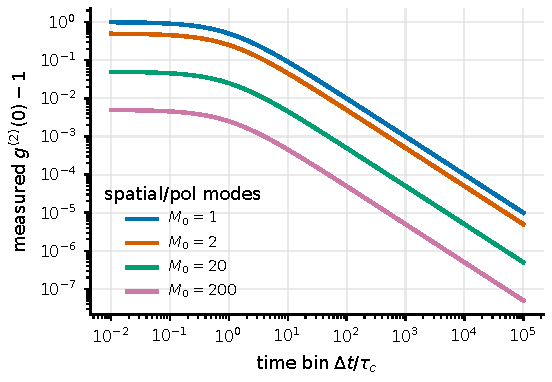
\includegraphics[width=0.82\linewidth]{figures/generated/chapter_09/ch09_thermal_mode_dilution.pdf}
\caption{The thermal-light bunching contrast falls as the effective number of modes rises. The horizontal axis is the ratio of the time bin to the coherence time, and \(M_0\) on the curves represents the number of spatial and polarization modes entering the same correlation estimator. Even if the source itself is pure thermal light, a wide time bin, mixing of multiple polarizations, and mixing of multiple spatial modes all pull \(g^{(2)}(0)-1\) toward zero: this is precisely the fundamental reason why photon-statistics fingerprints are so hard to see in astrophysical sources.}
\label{fig:e16-mode-dilution}
\end{figure}

Now overlay this dilution on the preceding picture and it becomes clear ``why it is extremely hard to isolate genuinely nonclassical light in astrophysical sources.'' First, most mechanisms \emph{by default} give chaotic thermal light (\(g^{(2)}(0)=2\)), and the candidates for nonclassical light (\(g^{(2)}(0)<1\)) can be counted on one's fingers. Second, even if some coherent mechanism in principle deviates from thermal statistics, mode dilution will compress the measurable deviation to \(10^{-2}\) or even lower. Third, even if your signal survives, instrumental and propagation effects will forge spurious correlations: dead time, afterpulsing, timestamp quantization, and trigger selection will rewrite the arrival-time correlation (a spurious \(g^{(2)}\) structure); plasma scintillation, scattering tails, gravitational microlensing, and frequency-dependent absorption will create cross-frequency correlations; a narrow maser line superposed on a thermal background, or a coherent pulse superposed on a synchrotron continuum, will make the mean spectrum look smooth while the photon statistics are no longer of a single kind. So any ``anomalous \(g^{(2)}\) peak'' must first be reconciled item by item against instrument, propagation, and mixed sources before one dares think ``nonclassical'' (Figure~\ref{fig:e16-g2-diagnostics} places the \(g^{(2)}(\tau)\) shapes of single-mode thermal light, multimode dilution, coherent state, and narrow coherent line side by side, precisely the reference figure for this item-by-item screening). The event tables, time-shifted backgrounds, and covariance estimates of Chapters~\ref{chap:e13} and~\ref{chap:e14} provide exactly the analysis layer needed for such item-by-item screening.

\begin{figure}[tbp]
\centering
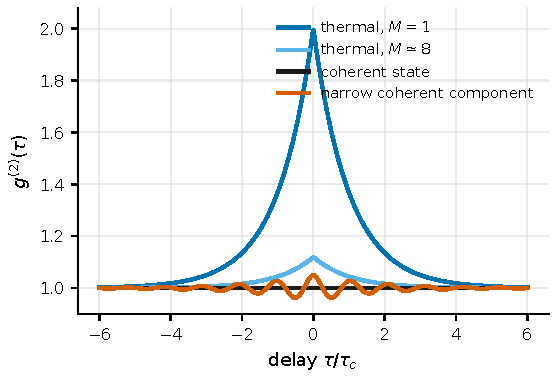
\includegraphics[width=0.82\linewidth]{figures/generated/chapter_09/ch09_radiation_g2_diagnostics.pdf}
\caption{\(g^{(2)}(\tau)\) for different light fields. Single-mode thermal light gives a bunching peak of height 2 at zero delay; multimode averaging lowers the peak (Eq.~\eqref{eq:e16-mode-dilution}); an ideal coherent state approaches 1; a narrow coherent spectral line or stimulated component can leave a small oscillation or narrow peak on a near-Poisson background. The horizontal axis is normalized to the coherence time \(\tau_c\).}
\label{fig:e16-g2-diagnostics}
\end{figure}

The correct posture for mechanism judgment is thus to gather all measurable quantities into the same observation vector for joint diagnosis, rather than staring at the mean spectrum alone:
\begin{equation}
  \bm{d}=
  \left\{
  I_\nu(t),\,
  Q_\nu(t),U_\nu(t),V_\nu(t),\,
  g^{(2)}_{ab}(\tau;\nu_i,\nu_j),\,
  \Delta t_{\rm var},\,
  \Omega_{\rm s}
  \right\}.
  \label{eq:e16-diagnostic-vector}
\end{equation}
\begin{formulaexplain}
\(\bm{d}\) the mechanism-diagnostic observation vector; it simultaneously collects intensity, Stokes polarization, second-order correlation, variability timescale, and angular scale. Mechanism judgment must rely on these quantities \emph{jointly}; the mean spectrum alone is not enough.
\end{formulaexplain}
where \(Q,U,V\) are the Stokes parameters, the subscripts \(a,b\) label telescope, polarization, or frequency channel, \(\Delta t_{\rm var}\) is the variability timescale, and \(\Omega_{\rm s}\) is the angular-scale constraint. Placing each mechanism in this vector separates the fingerprints: a thermal source (low polarization, finite \(T_b\), and residual-after-dilution thermal bunching); optically thin synchrotron (high linear polarization, power-law spectrum); maser (narrow line, extremely high \(T_b\), strong polarization); FRB (extremely high \(T_b\), millisecond-to-microsecond structure, dispersion, strong polarization). And scattering and plasma propagation change the temporal structure and spectrum, yet should \emph{not} be mistaken for the emission statistics of the source itself. Figure~\ref{fig:e16-diagnostic-plane} draws two of these axes (brightness temperature, polarization fraction, with point size indicating the measurable second-order coherence contrast) into a diagnostic plane, helping us locate at a glance which class of mechanism a source roughly falls into.

\begin{figure}[tbp]
\centering
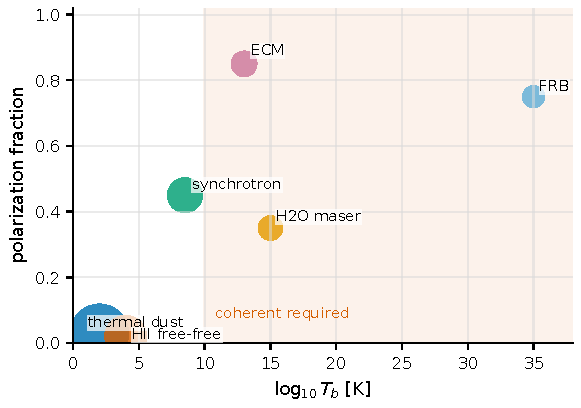
\includegraphics[width=0.86\linewidth]{figures/generated/chapter_09/ch09_diagnostic_plane.pdf}
\caption{The joint diagnostic plane of radiation mechanisms. The horizontal axis is brightness temperature, the vertical axis polarization fraction, and point size indicates the order of magnitude of the measurable second-order coherence contrast. Thermal dust and HII regions sit in the low-brightness-temperature, low-polarization region; synchrotron radiation has higher polarization but a brightness temperature usually below that of coherent bursts; the electron-cyclotron maser, molecular masers, and FRBs enter the high-brightness-temperature region and require coherent emission, pumping, or charge bunching to explain.}
\label{fig:e16-diagnostic-plane}
\end{figure}

\section{Chapter Summary}
\label{sec:e16-summary}

\begin{itemize}
  \item \textbf{The one-sentence main thread.} Translate radiation mechanisms into ``occupation number + photon statistics'': the mean spectrum \(I_\nu\) is only first-order information; the photon-arrival correlation (\(g^{(2)}\)), the polarization correlation, and the cross-frequency joint probability are the true fingerprints of the mechanism.
  \item \textbf{Brightness temperature is the occupation number.} Under the Rayleigh--Jeans definition, \(\bar n_\nu=k_BT_b/(h\nu)\) holds exactly (Eq.~\eqref{eq:e16-occupation-from-tb}). Stellar visible light has \(\bar n_\nu\sim10^{-2}\) (dilute), while an FRB has \(\bar n_\nu\sim10^{36}\) (cooperative). The incoherent-radio brightness-temperature limit is about \(10^{9}\)--\(10^{10}~{\rm K}\); exceeding it requires a coherent mechanism.
  \item \textbf{Thermal and nonthermal both default to chaotic light.} As long as ``many independent emitters add up, with random phase within a narrow band,'' the field is a Gaussian process, and the Siegert relation gives single-mode \(g^{(2)}(0)=2\) (Eq.~\eqref{eq:e16-siegert}). Blackbody, free-free, synchrotron, inverse-Compton: the spectra and polarizations differ, but the photon statistics belong to the same chaotic-thermal-light setting.
  \item \textbf{Only coherent mechanisms may deviate.} Masers/lasers rely on population inversion and stimulated emission; coherent curvature radiation relies on charge bunching (power \(\propto N^2\)). They break the premise of ``independent addition,'' and the occupation number and brightness temperature break through the ceiling, but an astrophysical maser is not the same as a laboratory single-mode laser.
  \item \textbf{Nonclassical light is extremely hard to isolate.} Mode dilution (Eq.~\eqref{eq:e16-mode-dilution}) compresses \(g^{(2)}_{\rm meas}(0)-1\sim1/M_{\rm eff}\) to \(10^{-2}\) or even lower; candidate mechanisms are already scarce; and instrumental and propagation effects can still forge correlations. Mechanism judgment must use the joint diagnostic vector~\eqref{eq:e16-diagnostic-vector} and reconcile the data with the screening tools of Chapters~\ref{chap:e13} and~\ref{chap:e14}.
\end{itemize}

\noindent\textbf{Questions to Ponder.} (1) For a star, the radio end and the optical end have the same matter temperature; why do their occupation numbers \(\bar n_\nu\) differ by several orders of magnitude? (2) The synchrotron spectrum is a power law and its polarization can reach 70\%; on what grounds do we say its photon statistics belong to the same setting as a blackbody? (3) If you see \(g^{(2)}(0)=1.01\) in the data, what are at least three classes of spurious signal you must rule out before concluding ``bunching detected''?
